\documentclass[10pt,a4paper]{article}
\usepackage[margin=1.7cm]{geometry}
\usepackage[T1]{fontenc}
\usepackage[utf8]{inputenc}
\usepackage[italian]{babel}
\usepackage{amsmath,amssymb,booktabs,graphicx,hyperref,array}
\title{Sezione numerica: Allen--Cahn con bordo dinamico e minimizzazione WED}
\author{Sezione autonoma di verifica numerica}
\date{22 ottobre 2026}
\begin{document}
\maketitle

\section{Modello, discretizzazione e implementazione}
Si considera il sistema parabolico adimensionale
\begin{align*}
 u_t-\Delta u+u^3-u&=0 &&\text{in }\Omega\times(0,T),\\
 u_{\Gamma,t}-\Delta_\Gamma u_\Gamma+\beta(u_\Gamma^3-u_\Gamma)&=-\partial_nu
 &&\text{su }\Gamma\times(0,T),\\
 u_\Gamma&=u|_\Gamma,
\end{align*}
con $\Omega=(0,2)\times(0,1)$ e $\Gamma=\partial\Omega$. Il parametro $\beta>0$ pesa il potenziale di reazione superficiale; nel bulk il potenziale resta $F(u)=\frac14(u^2-1)^2$, mentre sul bordo è $G(u_\Gamma)=\frac{\beta}{4}(u_\Gamma^2-1)^2$. L'energia considerata è
\[
 E(t)=\frac12\int_\Omega|\nabla u|^2+\int_\Omega F(u)
 +\frac12\int_\Gamma|\nabla_\Gamma u_\Gamma|^2+\int_\Gamma G(u_\Gamma).
\]
Tutte le quantità sono adimensionali. OOFEM C++ risolve il problema diretto; il minimizzatore WED è un programma Python separato che legge la mesh dall'input OOFEM, assembla il funzionale e non è eseguito dall'eseguibile C++.

Gli elementi spaziali sono quadrilateri bilineari Q1 con la stessa variabile scalare condivisa fra bulk e bordo; gli elementi di bordo sono segmenti lineari. Si usano nove punti di Gauss sui quadrilateri per integrare la reazione cubica Q1 e tre punti sugli elementi di bordo. Il solver diretto usa l'integratore implicito OOFEM con $\alpha=1$; nei test MMS il passo è $\Delta t=5\,10^{-4}$ e il criterio lineare/nonlineare dichiarato nell'input è $\mathrm{rtol}=10^{-11}$. Nel WED la traiettoria è approssimata con elementi lineari nel tempo, quadratura di Gauss, terminale libero e Newton sparso smorzato. Si indica con $S_{\max}$ l'orizzonte nella variabile riscalata $s=t/\varepsilon$; il passo fisico è $\Delta t=\varepsilon\Delta s$. La tolleranza WED riportata è la norma infinito del gradiente del funzionale riscalato, con massimo 100 iterazioni.

Per il test non uniforme si usa
\[
 u_0(x,y)=0.2+0.1\left[\cos\!\left(\frac{\pi x}{2}\right)\cos(\pi y)
 +0.25\sin\!\left(\frac{\pi x}{2}\right)\sin(\pi y)\right],
\]
con $\beta=1$ e sorgente MMS disattivata. Il funzionale WED troncato è
\[
 J_\varepsilon(u)=\int_0^{S_{\max}}e^{-s}\left[\frac12\|u_s\|^2_{L^2(\Omega)\oplus L^2(\Gamma)}
 +\varepsilon\left(\frac12\|\nabla u\|^2_{L^2(\Omega)}+\frac12\|\nabla_\Gamma u_\Gamma\|^2_{L^2(\Gamma)}
 +\int_\Omega F(u)+\int_\Gamma G(u_\Gamma)\right)\right]ds,
\]
con $u(0)=u_0$. L'implementazione numerica minimizza una versione riscalata di questo funzionale; la moltiplicazione per una costante positiva non ne cambia il minimizzatore.

\begin{figure}[ht]\centering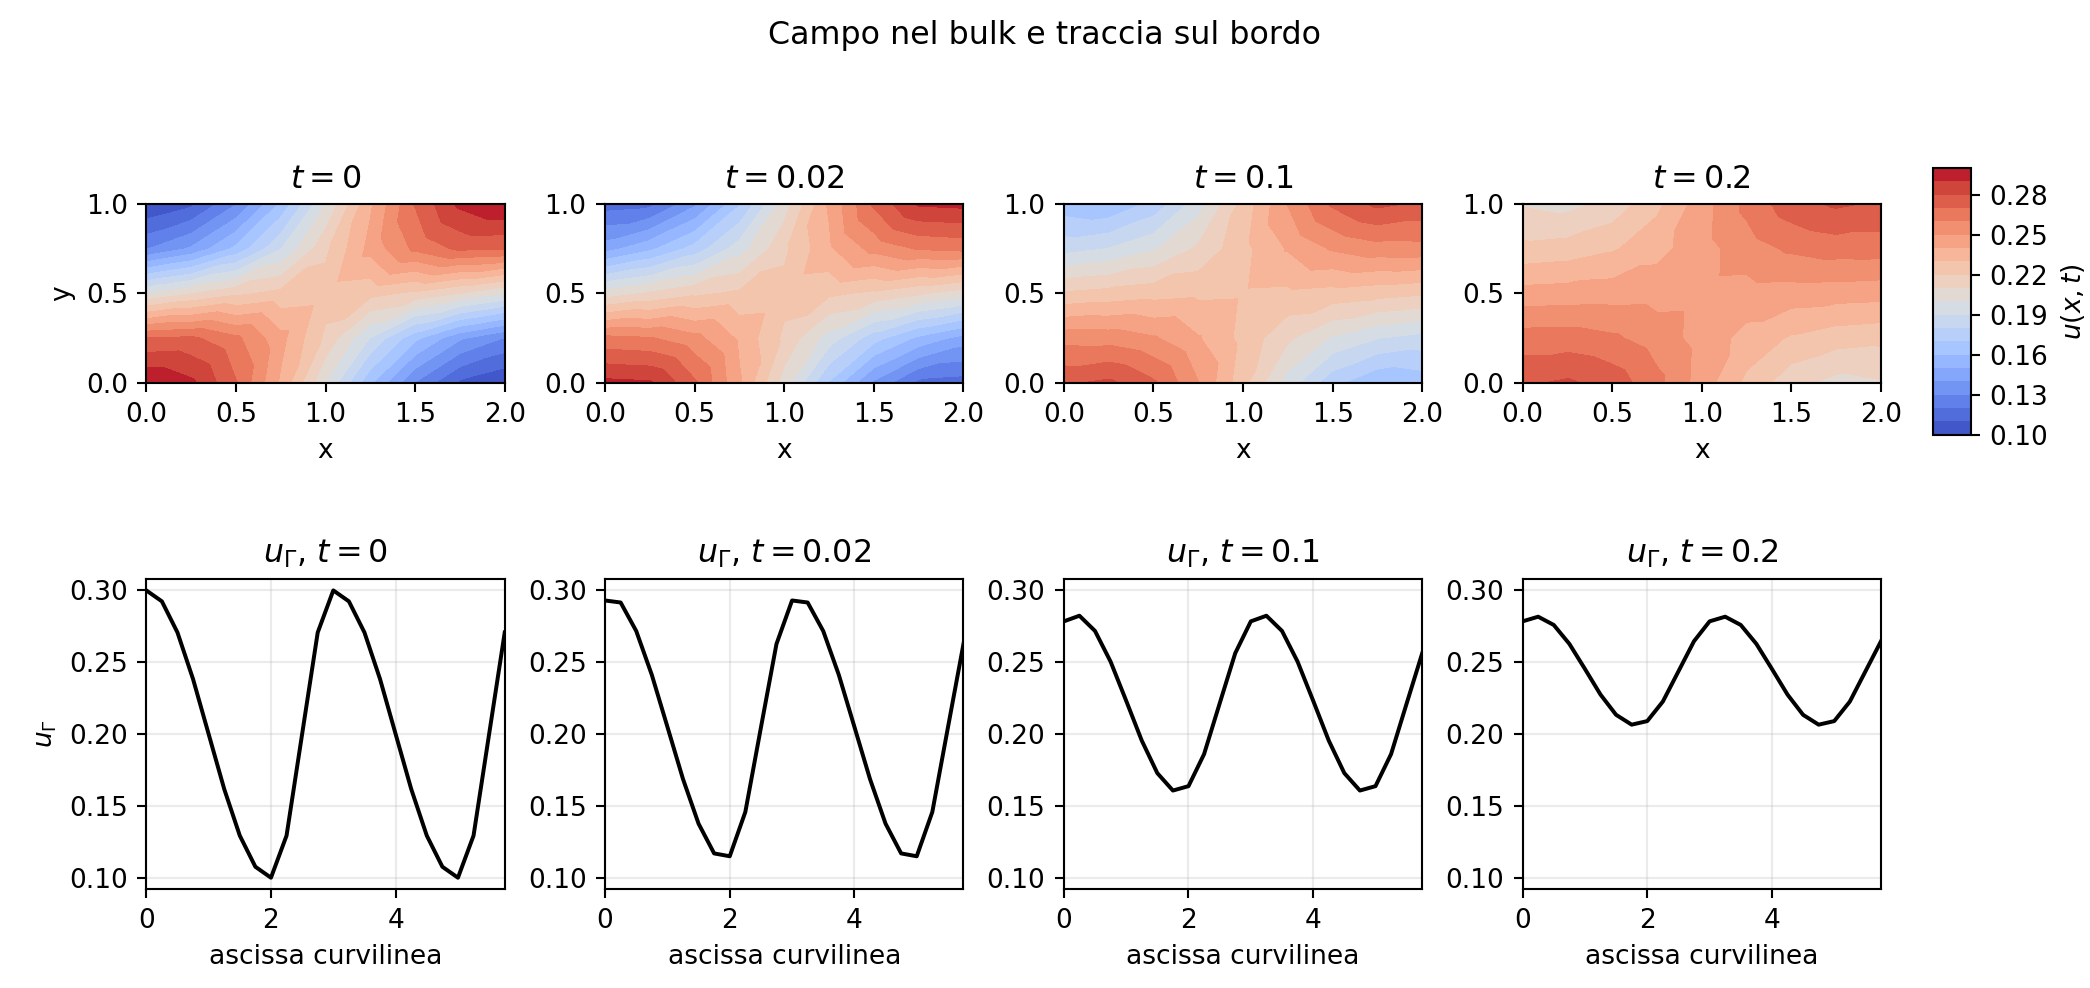
\includegraphics[width=.96\linewidth]{paper_figures/figure1_field_boundary.png}\caption{Snapshot del campo bulk e profilo della traccia sul bordo a $t=0,0.02,0.1,0.2$ per il benchmark non uniforme su $[0,2]\times[0,1]$, mesh $8\times4$, sorgente MMS disattivata e $\beta=1$.}\label{fig:field}\end{figure}

\section{Verifica del solver diretto: soluzione fabbricata}
La verifica MMS usa il campo esatto
\[
 u^*(x,y,t)=0.2+0.1e^{-t}\left[\cos\!\left(\frac{\pi x}{2}\right)\cos(\pi y)
 +0.25\sin\!\left(\frac{\pi x}{2}\right)\sin(\pi y)\right]
\]
e sorgenti fabbricate coerenti nel bulk e sul bordo, con $\beta=1$. Si misura l'errore RMS nodale al tempo $T=0.02$; $h$ è il lato delle celle quadrilatere. La pendenza $p=\log_2(e_h/e_{h/2})$ è una stima empirica.
\begin{center}\small
\begin{tabular}{rrrrrrr}
\toprule
mesh & nodi/DoF & $h$ & RMS nodale & massimo assoluto & $\Delta t$ & $p$\\
\midrule
$8\times4$ &45&0.250&$7.8821\,10^{-5}$&$1.8014\,10^{-4}$&$5\,10^{-4}$&--\\
$16\times8$&153&0.125&$1.7886\,10^{-5}$&$3.8000\,10^{-5}$&$5\,10^{-4}$&2.140\\
$32\times16$&561&0.0625&$4.3869\,10^{-6}$&$9.4361\,10^{-6}$&$5\,10^{-4}$&2.028\\
\bottomrule
\end{tabular}
\end{center}
L'errore RMS è $\sqrt{N^{-1}\sum_{i=1}^N(u_i-u^*_i)^2}$. La convergenza osservata è compatibile con ordine spaziale due per questo solver diretto e questo MMS; non verifica il minimizzatore WED.

\section{Dissipazione e bilancio energetico discreto}
Si definiscono le dissipazioni bulk e superficiale
\[
 D_\Omega=\int_0^T\!\int_\Omega|u_t|^2,\qquad
 D_\Gamma=\int_0^T\!\int_\Gamma|u_{\Gamma,t}|^2,
\]
e il residuo $R_E=E(T)-E(0)+D_\Omega+D_\Gamma$. Il postprocessing stima $u_t$ con differenze all'indietro e integra le dissipazioni con le matrici di massa FEM. I tre run usano $T=0.1$, dominio $[0,1]^2$, mesh quadrilatera $20\times20$, dato iniziale $u_0(x,y)=0.1+0.05\cos(2\pi x)$, $\beta=1$ e sorgente MMS disattivata; si varia solo il passo. Questo è un controllo discreto a passo finito, non una dimostrazione analitica di stabilità.
\begin{center}\small
\begin{tabular}{rrrrrrr}
\toprule
$\Delta t$&$E(0)$&$E(T)$&$D_\Omega$&$D_\Gamma$&$R_E$&$|R_E|/E(0)$\\
\midrule
0.00500&1.284456&1.209120&0.022138&0.047763&$-5.4350\,10^{-3}$&0.004231\\
0.00250&1.284456&1.209018&0.022887&0.049612&$-2.9395\,10^{-3}$&0.002289\\
0.00125&1.284456&1.208967&0.023310&0.050636&$-1.5420\,10^{-3}$&0.001201\\
\bottomrule
\end{tabular}
\end{center}
Il residuo è negativo e il suo valore assoluto normalizzato diminuisce da $0.423\%$ a $0.120\%$ al raffinarsi del passo. Le dissipazioni sono approssimate numericamente, quindi non ci si attende che il residuo a passo finito sia nullo. La Figura~\ref{fig:energy} mostra separatamente energia bulk e superficiale e la loro somma; non si richiede monotonia ai singoli contributi. L'evoluzione energetica illustrata usa il caso non forzato su $[0,1]^2$, mesh $20\times20$, $u_0(x,y)=0.1+0.05\cos(2\pi x)$, $\beta=1$, $T=0.1$ e $\Delta t=0.00125$.

\section{Limite $\varepsilon\to0$ per i minimizzatori WED}
Si confrontano errori $L^2$ spazio-tempo rispetto alla traiettoria diretta OOFEM sulla stessa mesh $8\times4$, interpolando i risultati sulla finestra comune $t\in[0,0.1]$. Definiamo
\[
 E_\Omega=\left(\int_0^{0.1}\|u_{\rm WED}(t)-u_{\rm OOFEM}(t)\|^2_{L^2(\Omega)}dt\right)^{1/2},\quad
 E_\Gamma=\left(\int_0^{0.1}\|u_{\Gamma,\rm WED}(t)-u_{\Gamma,\rm OOFEM}(t)\|^2_{L^2(\Gamma)}dt\right)^{1/2}.
\]
Il riferimento diretto ha $\Delta t=0.001$. Nella prima serie si fissano $S_{\max}=12$, $\Delta s=0.1$ e tolleranza WED $2\,10^{-5}$: il passo fisico cambia secondo $\Delta t=\varepsilon\Delta s$. Nella seconda serie si fissa $\Delta t=0.005$ e si sceglie $\Delta s=0.005/\varepsilon$; quindi $S_{\max}$ e la tolleranza restano invariati ma cambia la risoluzione in $s$. Ogni riga converge in due iterazioni Newton.
\begin{center}\small
\begin{tabular}{rrrrrrr}
\toprule
serie&$\varepsilon$&$\Delta s$&$\Delta t$&$\varepsilon S_{\max}$&$E_\Omega$&$E_\Gamma$\\
\midrule
$\Delta s$ fisso&0.1000&0.100&0.0100&1.200&$1.8485\,10^{-3}$&$3.1960\,10^{-3}$\\
&0.0500&0.100&0.0050&0.600&$1.1511\,10^{-3}$&$2.0198\,10^{-3}$\\
&0.0250&0.100&0.0025&0.300&$6.8730\,10^{-4}$&$1.1978\,10^{-3}$\\
&0.0125&0.100&0.00125&0.150&$3.8735\,10^{-4}$&$6.6759\,10^{-4}$\\
$\Delta t$ fisso&0.1000&0.050&0.0050&1.200&$1.8475\,10^{-3}$&$3.1947\,10^{-3}$\\
&0.0500&0.100&0.0050&0.600&$1.1511\,10^{-3}$&$2.0198\,10^{-3}$\\
&0.0250&0.200&0.0050&0.300&$6.8614\,10^{-4}$&$1.1959\,10^{-3}$\\
&0.0125&0.400&0.0050&0.150&$3.8299\,10^{-4}$&$6.6022\,10^{-4}$\\
\bottomrule
\end{tabular}
\end{center}
La pendenza locale $p=\log(E_{\varepsilon}/E_{\varepsilon/2})/\log 2$ è empirica e non un ordine teorico. A passo $\Delta s$ fisso gli ordini locali bulk/bordo sono 0.68/0.66, 0.74/0.75 e 0.83/0.84; con $\Delta t$ fisico fisso sono circa 0.68/0.66, 0.75/0.75 e 0.84/0.86. Il trend decrescente è quindi simile nei due protocolli. Il controllo a passo fisico fisso riduce la confusione dovuta a $\Delta t$, ma non elimina ogni errore temporale; per $\varepsilon=0.0125$ esso comporta $\Delta s=0.4$.

Per valutare direttamente quest'ultimo effetto, si dimezza $\Delta s$ a $\varepsilon=0.0125$, lasciando fissi mesh, $S_{\max}=12$ e tolleranza $2\,10^{-5}$. Il numero di iterazioni rimane due. Gli errori rispetto a OOFEM variano di circa $0.9\%$ sia nel bulk sia sul bordo; la differenza fra le due traiettorie WED sulla stessa finestra è molto più piccola dell'errore totale:
\begin{center}\small
\begin{tabular}{rrrrrr}
\toprule
$\Delta s$&$\Delta t$&iterazioni&$E_\Omega$ vs OOFEM&$E_\Gamma$ vs OOFEM&scarto traiettoria WED bulk/bordo\\
\midrule
0.4&0.0050&2&$3.82985\,10^{-4}$&$6.60221\,10^{-4}$&riferimento\\
0.2&0.0025&2&$3.86483\,10^{-4}$&$6.66145\,10^{-4}$&$4.16\,10^{-6}/6.44\,10^{-6}$\\
\bottomrule
\end{tabular}
\end{center}
Il trend in $\varepsilon$ è stabile a questa verifica temporale mirata, mentre la variazione dell'errore contro OOFEM non è monotona nel raffinamento del solo passo. Non si interpreta pertanto la pendenza come ordine asintotico del metodo.

\begin{center}\small
\begin{tabular}{rrrrrr}
\toprule
$\Delta s$&$\Delta t=\varepsilon\Delta s$&iterazioni&$E_\Omega$&$E_\Gamma$&scarto WED vs $\Delta s=0.4$\\
\midrule
0.4&0.0050&2&$3.82985\,10^{-4}$&$6.60221\,10^{-4}$&riferimento\\
0.2&0.0025&2&$3.86483\,10^{-4}$&$6.66145\,10^{-4}$&$4.16\,10^{-6}/6.44\,10^{-6}$\\
\bottomrule
\end{tabular}
\end{center}

\begin{figure}[ht]\centering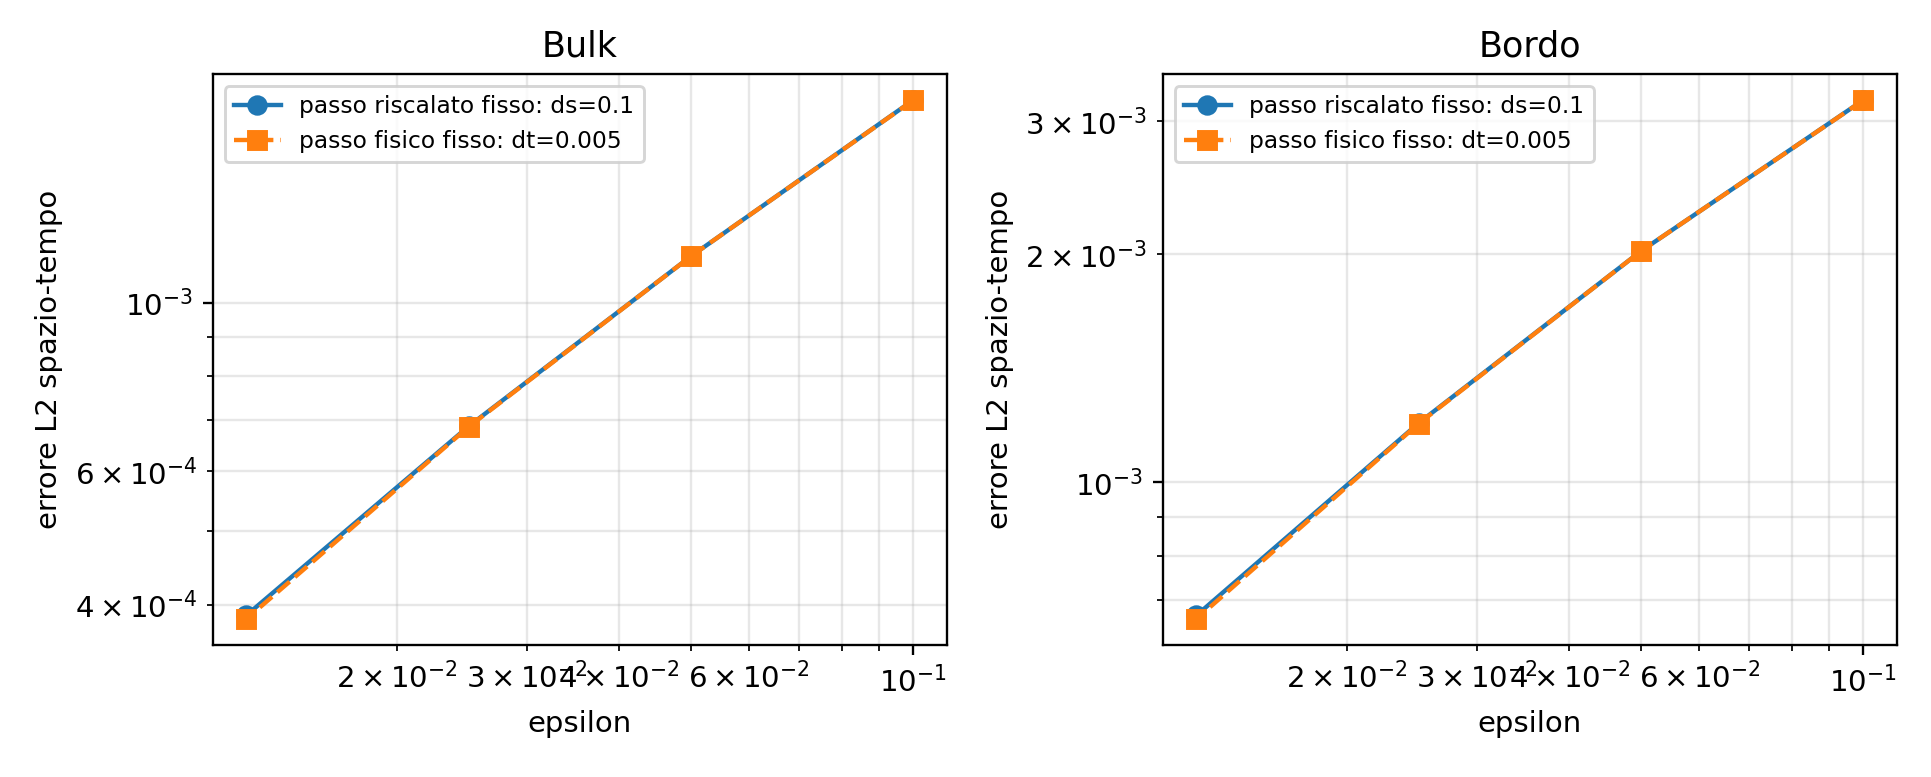
\includegraphics[width=.96\linewidth]{paper_figures/figure2_epsilon.png}\caption{Errori bulk e di bordo contro $\varepsilon$. Linea continua: $\Delta s=0.1$; tratteggiata: $\Delta t=0.005$ fisso. Ogni errore è integrato sulla finestra fisica comune $[0,0.1]$ rispetto a OOFEM diretto ($\Delta t=0.001$).}\label{fig:epsilon}\end{figure}

\section{Sensibilità all'orizzonte e convergenza spaziale WED}
\subsection{Orizzonte troncato}
Con $\varepsilon=0.05$, $\Delta s=0.1$, tolleranza $2\,10^{-5}$ e mesh $8\times4$, si confronta $S_{\max}=6,12$ con $18$ sulla finestra $t\in[0,0.1]$. La RMS spazio-tempo è calcolata sui nodi come $[\int_0^{0.1}N^{-1}\sum_i|u_i^{S_{\max}}(t)-u_i^{18}(t)|^2dt]^{1/2}$; il massimo è il massimo scarto nodale sulla medesima finestra.
\begin{center}\small
\begin{tabular}{rrrr}
\toprule
$S_{\max}$&$\Delta t=\varepsilon\Delta s$&RMS vs $S_{\max}=18$&massimo scarto nodale\\
\midrule
6&0.005&$3.6689\,10^{-5}$&$3.0215\,10^{-4}$\\
12&0.005&$1.5575\,10^{-7}$&$1.1327\,10^{-6}$\\
18&0.005&0 (riferimento)&0 (riferimento)\\
\bottomrule
\end{tabular}
\end{center}
Questo è un test di sensibilità al troncamento per il dato iniziale e la finestra scelti, non una stima uniforme per altri casi.
\begin{figure}[ht]\centering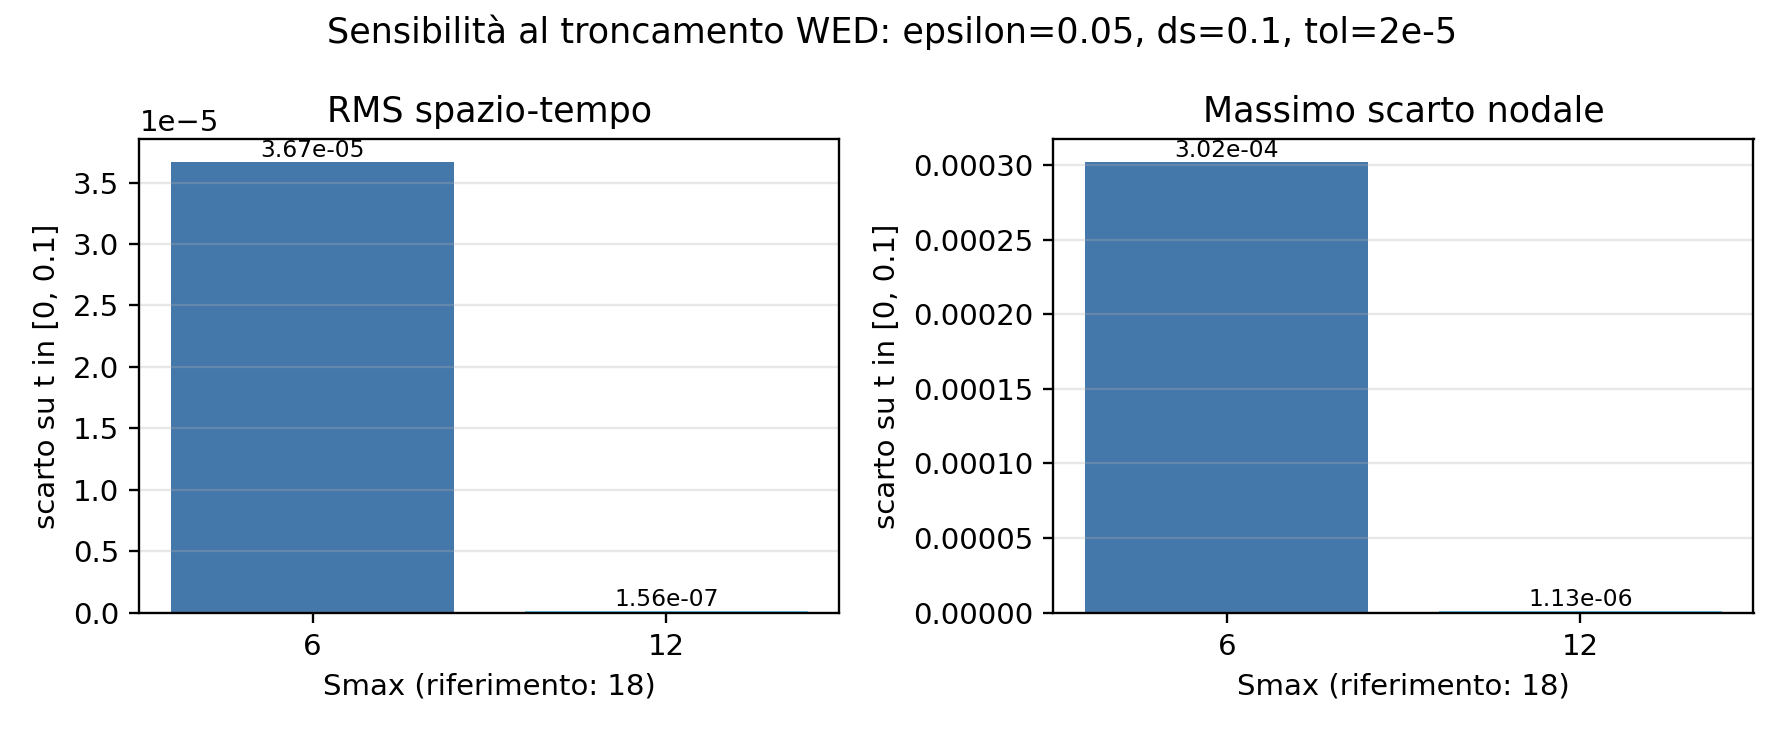
\includegraphics[width=.78\linewidth]{paper_figures/figure3_horizon.png}\caption{Scarti RMS e massimo nodale rispetto alla traiettoria con $S_{\max}=18$, per $\varepsilon=0.05$, $\Delta s=0.1$ e $t\in[0,0.1]$.}\label{fig:horizon}\end{figure}

\subsection{Raffinamento della mesh}
Si confrontano traiettorie WED a $\varepsilon=0.05$ con la soluzione WED sulla mesh $32\times16$ come riferimento numerico. Le norme spazio-tempo sono valutate su $t\in[0,0.1]$. Il run base usa $\Delta s=0.1$, tol $2\,10^{-5}$; il controllo usa $\Delta s=0.05$, tol $2\,10^{-6}$. La mesh fine non è una soluzione esatta. La tabella riporta gli errori rispetto al riferimento e gli ordini empirici bulk/bordo stimati usando le due mesh coarse.
\begin{center}\scriptsize
\begin{tabular}{llrrrrr}
\toprule
run&mesh&$h$&$E_\Omega$&$E_\Gamma$&$p_\Omega$&$p_\Gamma$\\
\midrule
base&$8\times4$&0.250&$2.1961\,10^{-4}$&$3.1175\,10^{-4}$&2.107&2.243\\
&$16\times8$&0.125&$5.0963\,10^{-5}$&$6.5835\,10^{-5}$&--&--\\
&$32\times16$&0.0625&0 (rif.)&0 (rif.)&--&--\\
raffinato&$8\times4$&0.250&$2.1977\,10^{-4}$&$3.0581\,10^{-4}$&2.108&2.216\\
&$16\times8$&0.125&$5.0972\,10^{-5}$&$6.5840\,10^{-5}$&--&--\\
&$32\times16$&0.0625&0 (rif.)&0 (rif.)&--&--\\
\bottomrule
\end{tabular}
\end{center}
La stima dell'ordine cambia di circa 0.001 nel bulk e 0.028 sul bordo fra i due settaggi: per queste griglie la tendenza è compatibile con ordine spaziale due ed è stabile al raffinamento temporale e del criterio di arresto. Il confronto WED/OOFEM contiene anche il bias a $\varepsilon>0$ e non viene usato per stimare l'ordine spaziale.
\begin{figure}[ht]\centering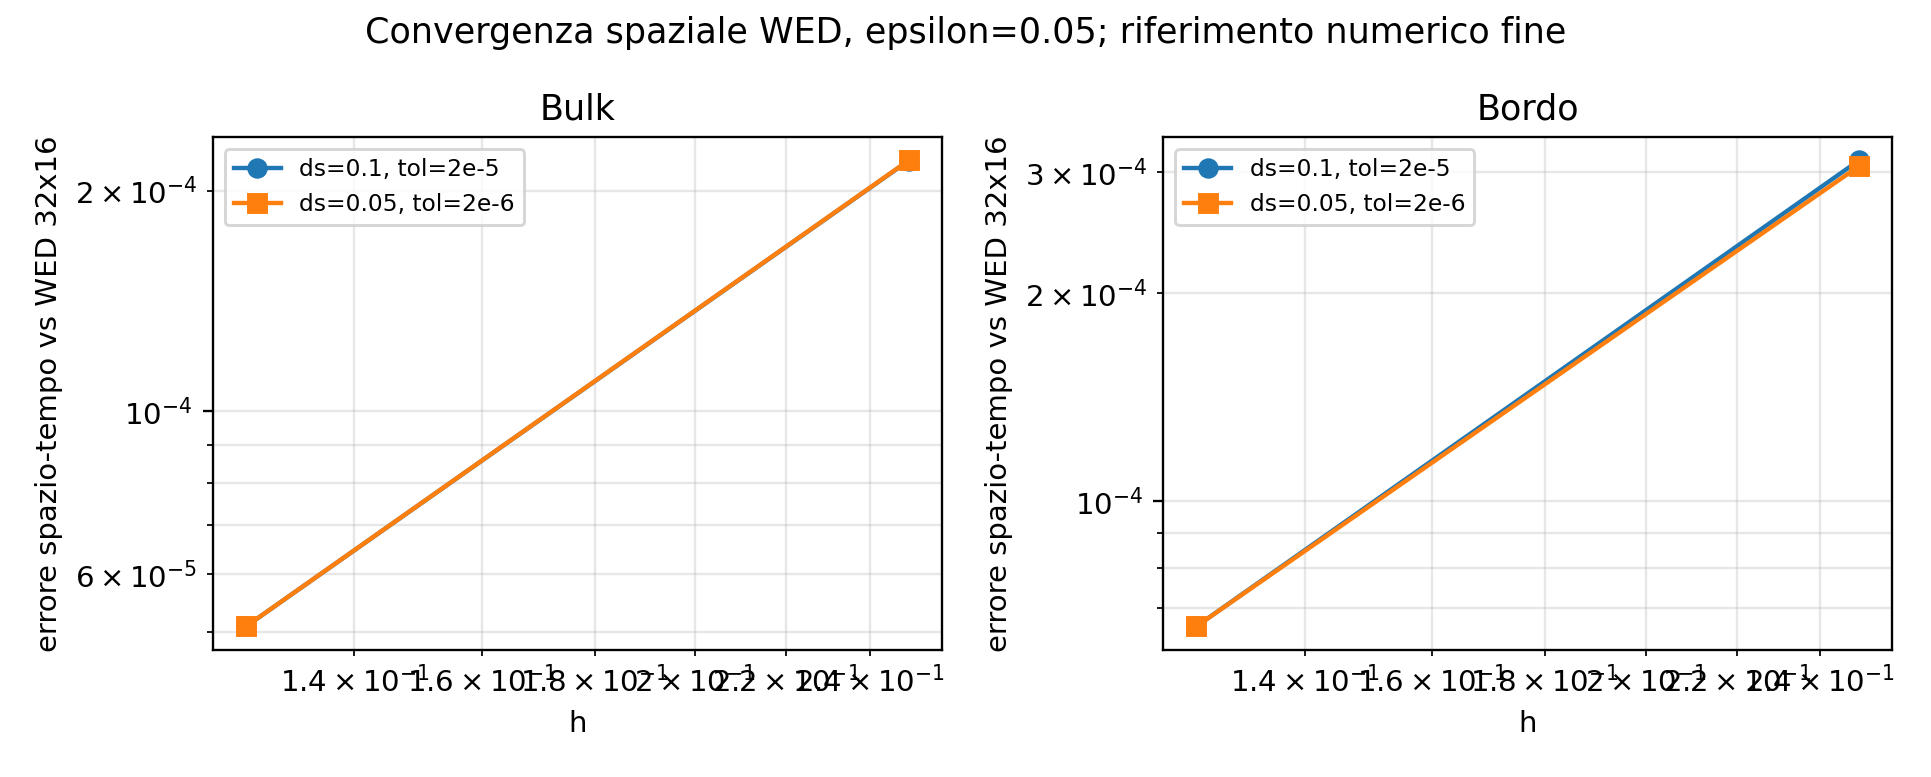
\includegraphics[width=.96\linewidth]{paper_figures/figure4_mesh.png}\caption{Errori bulk e superficiali rispetto alla traiettoria WED $32\times16$ a pari $\varepsilon$. La soluzione fine è un riferimento numerico; le due serie differiscono per $\Delta s$ e tolleranza come indicato in legenda.}\label{fig:mesh}\end{figure}

\begin{figure}[ht]\centering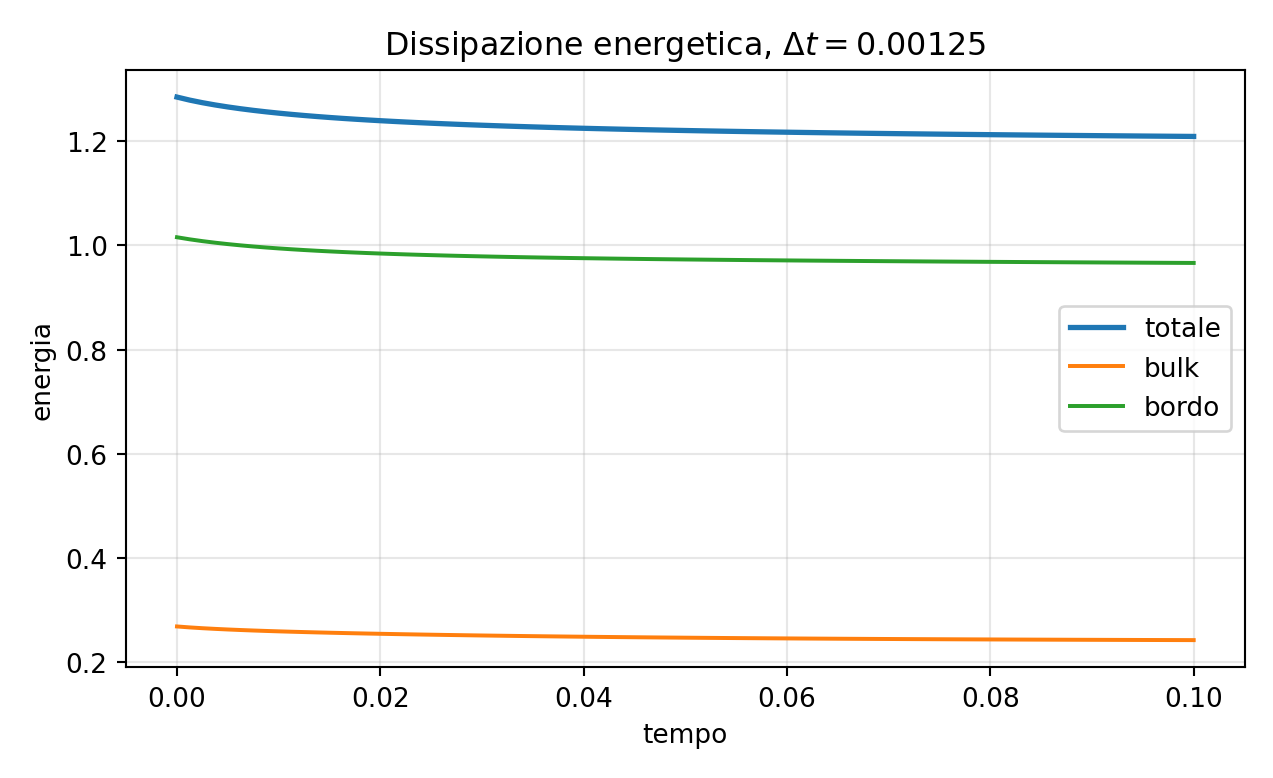
\includegraphics[width=.78\linewidth]{paper_figures/figure5_energy.png}\caption{Energia bulk, superficiale e totale per l'evoluzione diretta Allen--Cahn su $[0,1]^2$, mesh quadrilatera $20\times20$, $T=0.1$, passo $\Delta t=0.00125$, $\beta=1$. L'energia totale decresce; non si assume monotonia dei singoli contributi.}\label{fig:energy}\end{figure}

\section{Effetto del parametro $\beta$}
Si varia $\beta\in\{0.5,1,2,5\}$ mantenendo geometria $[0,2]\times[0,1]$, mesh $8\times4$, dato iniziale non uniforme definito sopra e sorgente MMS disattivata. La serie OOFEM usa $\Delta t=5\,10^{-4}$ fino a $T=0.02$; la serie WED usa $\varepsilon=0.05$, $S_{\max}=4$, $\Delta s=0.1$, tolleranza $2\,10^{-5}$ fino a $T=0.2$. Le serie hanno tempi finali diversi e sono mostrate separatamente, senza confronto punto a punto. $M_\Gamma(T)=|\Gamma|^{-1}\int_\Gamma u_\Gamma(T)$ è la media sul bordo.
\begin{center}\small
\begin{tabular}{rrrrrr}
\toprule
backend, $T$&$\beta$&$M_\Gamma(T)$&$E_\Gamma(T)$&$D_\Omega$&$D_\Gamma$\\
\midrule
OOFEM, 0.02&0.5&0.202747&0.739877&0.005098&0.018408\\
&1&0.204470&1.423137&0.005238&0.020230\\
&2&0.207956&2.783037&0.006023&0.029831\\
&5&0.218748&6.806088&0.012690&0.109610\\
WED, 0.2&0.5&0.220390&--&--&--\\
&1&0.233905&--&--&--\\
&2&0.264304&--&--&--\\
&5&0.382729&--&--&--\\
\bottomrule
\end{tabular}
\end{center}
L'energia $E_\Gamma$ e le dissipazioni nella tabella sono valutate per il transiente diretto; non sono riportate per WED in questa tabella. Si osserva una risposta a $\beta$ per il dato iniziale scelto, senza affermare monotonicità universale né un tempo di rilassamento.
\begin{figure}[ht]\centering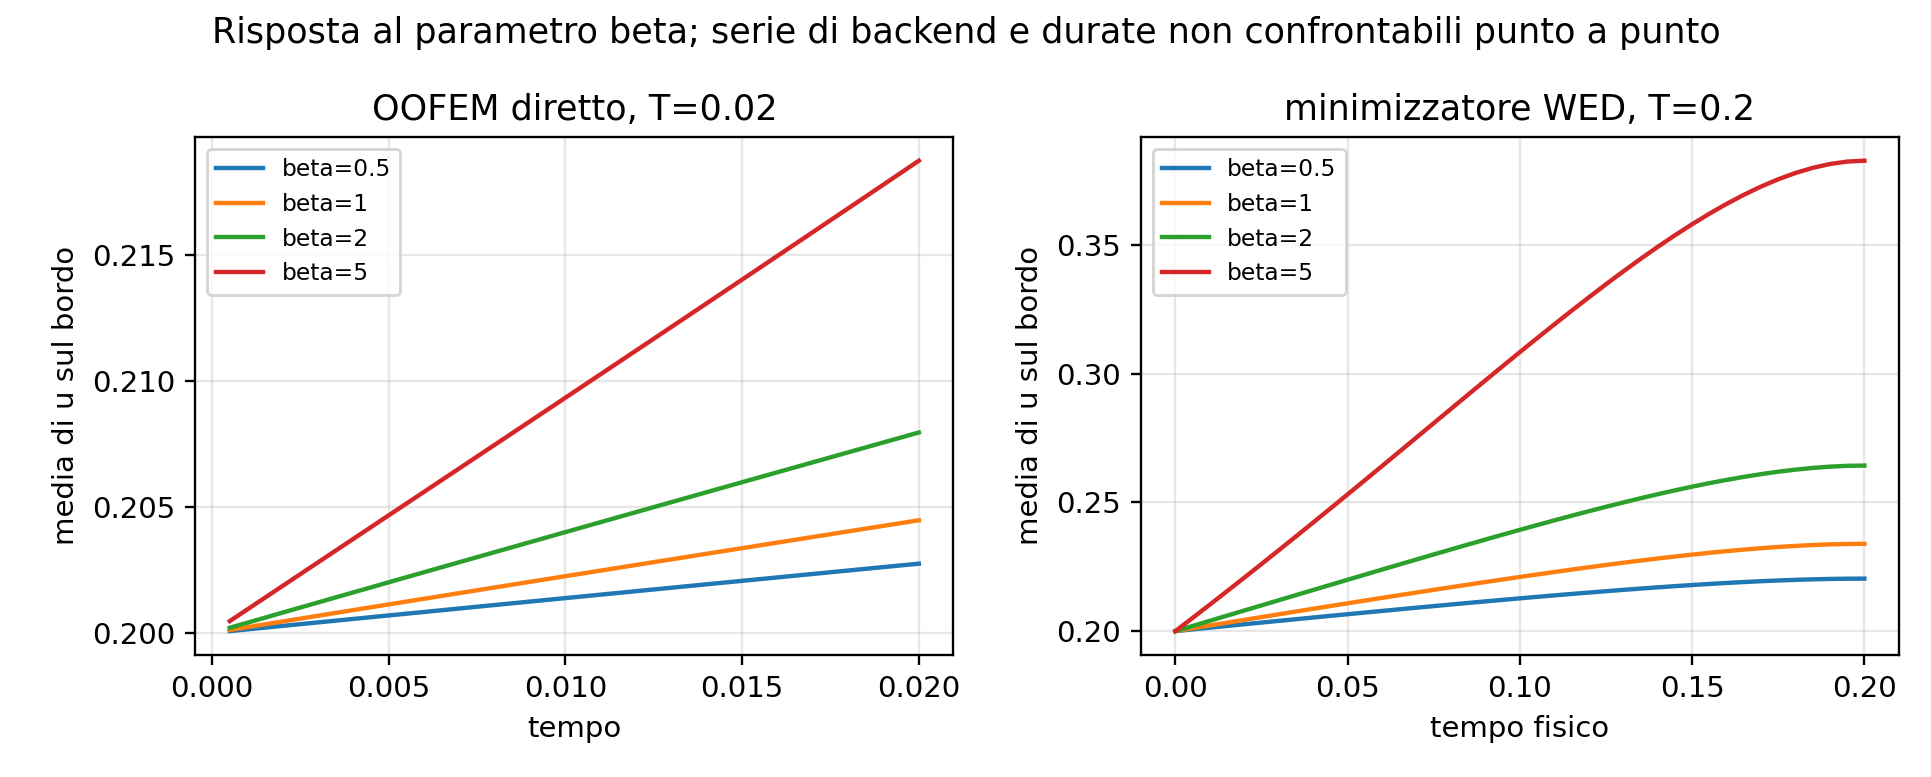
\includegraphics[width=.96\linewidth]{paper_figures/figure6_beta.png}\caption{Media di $u_\Gamma$ per $\beta=0.5,1,2,5$. Pannello sinistro: OOFEM diretto fino a $T=0.02$, $\Delta t=5\,10^{-4}$. Pannello destro: minimizzatore WED fino a $T=0.2$, $\varepsilon=0.05$, $S_{\max}=4$, $\Delta s=0.1$. I due pannelli hanno backend e durate differenti.}\label{fig:beta}\end{figure}

\section{Limiti e riproducibilità}
Il caso considerato è parabolico, bidimensionale e basato su quadrilateri Q1. Il benchmark triangolare P1 e la variante iperbolica a onde non sono inclusi. La MMS e il bilancio energetico sono verifiche del solver diretto, non del minimizzatore WED; i test di $\varepsilon$, orizzonte e mesh riguardano il backend WED separato. Gli ordini sono stime empiriche sui benchmark indicati. Il confronto WED/OOFEM include il bias di $\varepsilon$ e non è usato come convergenza mesh.

{\sloppy La riproduzione si basa sugli input, log, CSV e script archiviati in \texttt{doc/stvowu\_validation}; comandi, dipendenze e associazione fra risultati e driver sono documentati nel README. Il controllo energia usa differenze all'indietro sui campi salvati. Le conclusioni valgono per i dati, le mesh e i parametri riportati e non costituiscono validazione universale.\par}
\end{document}
